% This paper will be submitted to EUSPN15.

\documentclass[3p,times,procedia]{elsarticle}
\flushbottom
\usepackage{ecrc}
\volume{00}
\firstpage{1}
\journalname{Procedia Computer Science}
\runauth{Christophe Van Ginneken, Jef Maerien,
Christophe Huygens, Wouter Joosen, Danny Hughes}
\jid{procs}
\usepackage{amssymb}
\usepackage[figuresright]{rotating}

% additional packages and utility commands

\usepackage{float}

\newcommand{\TODO}{\textbf{\color{red}TODO}}

% \usepackage{flushend}

% while preparing, linenumbers come in handy
\usepackage{lineno}
\setlength\linenumbersep{1mm}
\linenumbers

% until we settle on the final name ;-)
\usepackage{xspace}
\newcommand{\NAME}{id-foo\xspace}

% http://tex.stackexchange.com/questions/299/how-to-get-long-texttt-sections-to-break
\newcommand*\justify{%
  \fontdimen2\font=0.4em% interword space
  \fontdimen3\font=0.2em% interword stretch
  \fontdimen4\font=0.1em% interword shrink
  \fontdimen7\font=0.1em% extra space
  \hyphenchar\font=`\-% allowing hyphenation
}

% http://en.wikibooks.org/wiki/LaTeX/Customizing_LaTeX
\newcommand{\ttt}[1]{\texttt{\justify{#1}}}

\usepackage{algpseudocode}
% custom Let command
\newcommand*\Let[2]{\State #1 $\gets$ #2}
\renewcommand{\algorithmicforall}{\textbf{for each}}
\let\ForEach\ForAll

\usepackage{listings}

\usepackage{tikz}
\usetikzlibrary{positioning}
\usetikzlibrary{calc}
\usetikzlibrary{graphs}
\usetikzlibrary{trees}
\usetikzlibrary{arrows}

\usepackage{tikz-3dplot}

%!TEX root=paper.tex

% basics

\tikzset{
  box/.style            = { rectangle, minimum width=2cm, minimum height=1cm },
  border/.style         = { thick, draw=black },
  round/.style          = { rounded corners=3mm },
}

% system

\tikzset{
  artifact/.style       = { box, font=\ttfamily },
  support/.style        = { box, font=\itshape },
  user/.style           = { artifact, fill=black!15!white },
  dom/.style            = { support,  fill=black!30!white },
  platform/.style       = { support,  fill=black!55!white, text=white },
  native/.style         = { support,  fill=black!70!white, text=white },
  generated/.style      = { artifact, border, dashed },
  resource/.style       = { artifact, border },
  representation/.style = { support, border, round }
}

% UML

\tikzset{
  class/.style={
    box,
    border,
    text centered,
    text width=1.75cm
  },
  relation/.style       = { thick, draw=black, <-},
  subclass/.style       = { relation, >=open triangle 60 },
  aggregate/.style      = { relation, >=open diamond },
  composite/.style      = { relation, >=diamond },
  dependency/.style     = { relation, >=latex, -> }
}

\lstdefinelanguage{foo-lang}{
  emph={module,const,from,import,extend,with,after,do,function,@every,having,if,return},
  emphstyle={\textbf},
  morecomment=[l]{//},
  moredelim=[is][]{@@}{@@},       % temp solution to allow keywords without emph
  moredelim=[is][\emph]{!!}{!!}   % temp solution to hightlight #atoms
}


\usepackage[autostyle]{csquotes}

\usepackage{booktabs}
\usepackage{multirow}
\usepackage{stfloats}



\begin{document}

\begin{frontmatter}

\dochead{6th International Conference on Emerging Ubiquitous Systems and
Pervasive Networks, EUSPN-2015 and the 5th International Conference on Current
and Future Trends of Information and Communication Technologies in Healthcare,
ICTH 2015,}

\title{
\FOO: A framework for efficient source code generation\\
of detection algorithms for the Internet of Things
}

\author[]{Christophe Van Ginneken}
\author[]{Jef Maerien}
\author[]{Christophe Huygens}
\author[]{\\Wouter Joosen}
\author[]{Danny Hughes}

\address{
iMinds-DistriNet, KU Leuven, 3001 Leuven, Belgium\\
\{firstname.lastname\}@cs.kuleuven.be
}

\begin{abstract}

The ability to detect patterns in its usage is what makes \emph{things}
\emph{smart}. The more patterns it can detect, the more accurate its
operational results will be. However, supporting an adequate set of pattern
detection algorithms imposes significant overhead on resource-constrained
devices such as those in the Internet of Things. Manual fusion of the
algorithms reduces resource consumption by optimizing resource sharing, yet,
proves to be time-consuming, repetitive and error-prone. To address this
problem we propose \FOO, a framework for the generation of efficient detection
algorithms. It consists of a domain specific language and a code generator. The
language allows formally describing the intent of detection algorithms and
supports the generator in organizing the source code. As a case study, we apply
\FOO to the generation of an Intrusion Detection System for wireless sensor
nodes. A side-by-side comparison shows that \FOO-generated source code reduces
message passing overhead, execution time and memory footprint in comparison to
sequential calls into stand-alone implementations of the algorithms.

\end{abstract}

\begin{keyword}

IoT, Domain Specific Languages, Source Code Generation, Source Code
Optimization, Intrusion Detection, Context Awareness

\end{keyword}

\end{frontmatter}

\vspace*{-10pt}

\section{Introduction}

The Internet of Things (IoT), the mother of all ubiquitous and pervasive
networks, populates our daily lives with millions of internet-connected
\emph{smart things}: from smart watches that assist visually impaired
persons\cite{porzi2013smart} to monitoring systems for flood hazardous
areas\cite{hughes2006gridstix}. Their applications cannot be more diverse,
however they share one common concern: each of these \emph{things} is
resource-constrained, relying on a battery and operating with limited
processing power and memory.

Although their applications at first seem unrelated, under the hood they share
a common paradigm: pattern recognition. With the introduction of \emph{smart
things}, we want to augment our lives with information that is hard, or at
least time and resource consuming, to obtain otherwise. The ability to detect
patterns in its usage or its applied context, is what makes these \emph{things}
\emph{smart}. A watch that recognizes gestures can perform certain actions on
behalf of its wearer. That same watch can also detect a wet floor and notify
this hazard.

Monitoring human activities is an active research field for more than a
decade\cite{lara2013survey}, but with the advent of the IoT it now moves into
the real world. Equipped with wearables with numerous sensors, the
possibilities seem endless, but so are the number of detection and recognition
algorithms that have to run simultaneously on these small \emph{things}, to
support our augmented reality.

Another prime example of a class of algorithms that inhibit the same properties
related to pattern recognition is Intrusion Detection (ID). The vast number of
security related opportunities for attackers makes way for an equally sized
amount of ID algorithms, all with a similar structure, but largely independent
operation.

% scientific contribution

The contributions of this paper are threefold: The first contribution consists
in the formulation of a design pattern for detection/recognition algorithms for
IoT devices. This defines the target algorithms that fit our proposed
framework. The second contribution is a framework called \FOO.\@ It enables the
formal description of algorithms on a functional level and provides a code
generator producing source code for a given platform and configuration. This
way, \FOO also addresses the heterogeneous nature of both IoT and the
algorithms. The third contribution introduces functional code fusion (FCF) as a
source code generation paradigm to address the combination of algorithms. FCF
identifies common data and functions, and organizes code to eliminate redundant
iterations, tests and computations. Results show reduced usage of the wireless
radio, execution time and memory usage.

% structure

The remainder of this paper proceeds as follows: section \ref{problems}
identifies problems that arise when combining multiple algorithms in the
context of resource-constrained devices. Section \ref{pattern} formulates a
pattern common to the detection/recognition algorithms in the IoT context.
Section \ref{design} introduces our framework, its design and components. In
section \ref{evaluation} we apply our solution to case study related to ID,
showing an actual implementation and evaluation of the experimental results.
Section \ref{related} explores related work in the field of DSLs and code
generation. Finally, section \ref{conclusion} summarizes our findings, draws
conclusions and identifies topics for future work.

\section{Problems when combining multiple algorithms}
\label{problems}

Simply taking existing implementations of algorithms and calling them in
sequence, to allow them to perform their functionality, will in most cases
result in suboptimal code. Three prime examples on the source code level
illustrate this:

\vspace{-2mm}

\begin{description}

  \item[Loops] by themselves are not a problem, but different loops, that
  perform the same operations in sequence, can cause overhead. An example is
  the handling of messages: each algorithm parses each observed message on the
  network, processing the same byte stream, performing comparable operations to
  find similar patterns. These loops can also hold calls to poll sensor for
  their values. This results in an execution overhead, putting a strain on the
  power consumption.

\vspace{-2mm}

  \item[Common data] cross-cuts the different algorithms, that have to store
  the same information over and over again within their own scope. This results
  in a lot of duplicated information in memory, raising the hardware
  requirements.

\vspace{-2mm}

  \item[The network] allows algorithms to operate on a distributed scale.
  Scattered calls to a message sending function cause multiple accesses to the
  wireless radio, keeping it active and energy consuming more than strictly
  needed.

\end{description}

Two operational aspects are orthogonal to these problems and further amplify
them:

\vspace{-2mm}

\begin{description}
  
  \item[Reimplementing] algorithms manually to eliminate these issues is
  not a one-time cost. A release of a new version of an algorithm, or simply a
  reselection of algorithms, due to a changing requirements, can trigger it.
  Also, changing, or simply implementing the algorithms from scratch, holds the
  risk of making mistakes.

\vspace{-2mm}

  \item[The heterogeneity of IoT devices] results in different software stacks,
  each with for example their own network API\@. This partially explains why
  there are few implementations of algorithms readily available to developers:
  there is no single platform to target for researchers, which lowers the
  opportunity to reuse prior work.

\end{description}

\section{A Design Pattern for Detection/Recognition Algorithms}
\label{pattern}

The source code level problems that arise when combining multiple algorithms,
as presented in section \ref{problems}, are in fact inherent to the design
pattern that is the foundation for the type of algorithms we identify in
typical detection/recognition applications in IoT applications. The formulation
of such a design pattern will allow us to define a strategy for the
optimization of the combination of these algorithms. We start by extracting two
common activities of these algorithms: the collection of sensor values and the
evaluation of thresholds. Periodically collecting sensor values requires
preparing the hardware for value extraction, waiting for the value to become
available, reading the actual bytes, interpreting them into a meaningful value
and recording them for further analysis. This can be as simple as reading a
single byte, but can also be as complex as parsing a network message.

A single recorded sensor value hardly ever results in a decision. The
combination, often over time, of several of these values and the evaluation of
thresholds will be key to decide if a change in the environment requires an
action. Updating such statistics and evaluating the corresponding thresholds
should be distinct operations. Therefore this is a separate function that is
also periodically executed.

This decoupling of detection and decision is the core of the design pattern for
ID algorithms. Listing \ref{alg:pattern} presents the design pattern in
pseudo-code. Applying the pattern in the context of multiple algorithms,
extends its scope and a pattern such as described in listing
\ref{alg:application} will typically appear. The pattern calls the individual,
implementations in sequence in two situations: first, to collect sensor
readings, and secondly, at a regular interval to allow for internal
housekeeping, such as threshold evaluation.

We clearly see the three aforementioned problems manifest itself: first, the
nesting of loops causes redundant executions of potentially the same sensor
readings inside the individual algorithms' $collect\_data$ functions. Second,
each individual algorithm stores the same sensor values in memory. Third,
scattered calls to e.g. network functions (in case of distributed algorithms)
lead to suboptimal use of the wireless radio.

Implementing the solution from scratch, it would be possible to identify these
problems and reorganize the code in such a way that sensor values are only read
once, stored in memory once and network messages parsed once. In section
\ref{problems} we identified two operational problems that show that this is
not feasible or at least suboptimal. We therefore present \FOO, a framework
that enables formally describing such algorithms and fusing common data and
functions in an automated way, to overcome both these problems.

\vspace{-2mm}

\begin{algorithm}[b]
  \caption{Detection/Recognition Algorithm Pattern}
  \label{alg:pattern}
  \begin{algorithmic}
    \Require{readings: global variables to hold collected sensor data for the given algorithm}
    \Require{devices: global variable to information about neighbor devices} \Comment{optional in case of distributed algorithms}
    \Function{collect\_data}{}
      \ForEach{$sensor \in required\_sensors$}
        \Let{values[]}{$sensor$}   \Comment{collect sensor data}
        \Let{$reading_{sensor}$}{\Call{interpret}{values[]}}  \Comment{update interpreted sensor info}
      \EndFor
      \State \Call{send}{$devices_x$, ``info''} \Comment{optionally exchange info} \label{alg:id-algo-pattern-send1}
    \EndFunction
    \Function{do\_housekeeping}{}
      \ForEach{$reading \in readings$} \label{alg:id-algo-pattern-loop2} \label{alg:id-algo-pattern-common-data}
        \If{$reading > \dots$} \Comment{validate recorded value}
          \State \dots \Comment{take actions}
          \State \Call{send}{$device_x$, ``info''} \Comment{optionally communicate} \label{alg:id-algo-pattern-send2}
        \EndIf
      \EndFor
    \EndFunction
  \end{algorithmic}
\end{algorithm}

\begin{algorithm}[b]
  \caption{Application pattern of multiple algorithms}
  \label{alg:application}
  \begin{algorithmic}
    \ForEach{$algorithm \in algorithms$}
      \State \Call{algorithm.collect\_data}{}
    \EndFor
    \ForEach{$algorithm \in algorithms$}        \Comment{at a given interval}
      \State \Call{algorithm.do\_housekeeping}{}
    \EndFor
  \end{algorithmic}
\end{algorithm}

\section{Design}
\label{design}

The previous sections identified loops, common data and the network as three
important code-level problems. These problems are inherent to detection
algorithms, but conflict with the target environment, the IoT\@. \FOO provides
a framework to efficiently implement these algorithms for the IoT and offers a
solution for all identified problems. It consists of a 1) DSL, 2) source code
generator and 3) software library. Figure \ref{fig:design} visualizes the
design.

\begin{figure}[b]
  \centering
  \scalebox{0.75}{
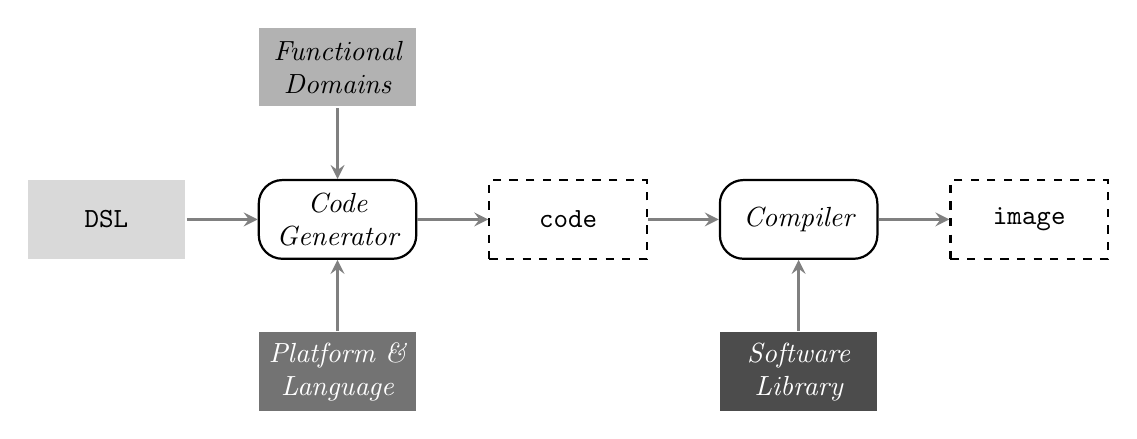
\begin{tikzpicture}[
  node distance=9mm,
  ,>=stealth,very thick,black!50,text=black,
  every new ->/.style={shorten >=1pt}
]
  \node (dsl)     [user]                                      {DSL};
  \node (cg)      [representation,right=of dsl,align=center]  {Code\\Generator};
  \node (code)    [generated,right=of cg]                     {code};
  \node (comp)    [representation,right=of code]              {Compiler};
  \node (image)   [generated,right=of comp]                   {image};

  \node (domains) [dom,above=of cg, align=center]             {Functional\\Domains};
  \node (plat)    [platform,below=of cg,align=center]         {Platform \&\\Language};          
  \node (lib)     [native,below=of comp,align=center]         {Software\\Library};

  \draw [->] (dsl)     -> (cg);
  \draw [->] (domains) -> (cg);
  \draw [->] (plat)    -> (cg);
  \draw [->] (cg)      -> (code);
  \draw [->] (code)    -> (comp);
  \draw [->] (lib)     -> (comp);
  \draw [->] (comp)    -> (image);
\end{tikzpicture}
}
\caption{The high level design of \FOO, showing the resources, processes and
artifacts. A grayscale background represents the level of platform dependency,
with darker shades indicating a higher dependency. Both the source code and the
installable image are artifacts.}
\label{fig:design}
\end{figure}

The DSL enables researchers to formally describe algorithms, without focusing
on any specific language or platform. A code generator can avoid the identified
problems concerning loops, common data and network access, as the formal
description provides the underlying intent, not the technical implementation.
It can also target different languages and platforms, while reusing a software
library that provides services including parsing, network access wrapping,\dots
It applies the Functional Code Fusion (FCF) paradigm to identify the hotspots
for optimization. A key component of FCF is the introduction of
\emph{functional domains} that harbor common functionality.

Using a DSL and code generator defines a development strategy. We will first
position \FOO and motivate its design. Second, we will look at the principal
design components of the DSL.\@ Third, we discuss the structure of the code
generator and introduce its software library, that offers a way to deal with
for example the network access issue.

\vspace{-1mm}
\subsection{\FOO as a Development Strategy}
\label{positioning}

The introduction of a code generator in the development process changes the way
of working. The actual source code is no longer the driving force, controlled
by developers. It is literally an intermediate representation between code
generator and compiler. A code generator constructs this representation using
three components, as shown in figure \ref{fig:design}: 1) the description of
the algorithm in the DSL, 2) information about the functional domains, and 3)
information about the platform and target language. At the level of the
compiler, a software library offloads specialized implementations and allow
custom extensions. The applied grayscale indicates the components' platform
dependency. This hierarchy is important from a development effort point of
view. The level of dependency on the target platform dictates the level of
effort to implement changes. This is important in relation to the scalability
of the framework itself.

\vspace{-1mm}
\subsection{\FOO as a Domain Specific Language}
\label{dsl-design}

It's important to remember that a DSL is merely a \emph{thin veneer over a
(semantic) model} \cite{fowler2010domain}. Its sole purpose should be
populating the model. \FOO's DSL and model focus on avoiding constructions that
result in problems concerning loops, common data and the use of the network. To
do this, \FOO uses an event-based approach to defining functionality.
Describing algorithms in function of events that occur will remove the
technical descriptions and allows FCF to identify the actual intent of the
algorithms with respect to the identified source code problems.

\vspace{-1mm}
\subsubsection{Loops}

Loops are a major contributor to the problem of algorithm fusibility. Loops in
program code are technical constructs and in fact often hide the intended
functionality. The example of parsing network messages illustrates this. Each
algorithm deals with parsing in the same way: loop over the bytes in the
payload and look for a pattern that identifies what the algorithm is looking
for. This is in fact a technical implementation choice. The underlying
functional intent is to react when such a pattern is present in a message. The
loop has \emph{activated} this functionality, but the real goal is to
\emph{passively} react on an event, not \emph{actively} look for it. Event
handling therefore can transform constructions with loops to their functional
meaning, allowing identification and fusion of common functionality.

\vspace{-1mm}
\subsubsection{Common Data}

Different detection algorithms typically deal with the same classes of
information, be it sensor data or network messages. Functional domains
consolidate these and store and manage this data in a unified way. \FOO
provides the concept of such domains as plug-ins to the DSL, extending it with
domain specific storage and logic. For example in the case of distributed
algorithms, such as ID algorithms, a \emph{Nodes} domain will manage
information about neighbor nodes, exposing them as global objects to the
algorithms, relieving them from managing these themselves. Functional domains
are accessible as collections, allowing execution of functions in their scope,
eliminating the need for explicit loops.

\vspace{-1mm}
\subsubsection{Unified Messaging}
\label{dsl-unified-msg}

Access to the network, scattered around an algorithm, causes the wireless radio
to be more active than needed. Delaying the sending of messages and grouping
them can lower this overhead. Sending and receiving of network messages is
tightly integrated with the previously mentioned concepts of event handling and
for example the Nodes domain. An underlying software library can handle all
interaction with the network, triggering functions by means of events when
parsing new messages and exposing an API to send messages through the Nodes
domain. This approach gives the framework complete control over communication
and allows for optimized marshaling and grouping of messages.

\vspace{-1mm}
\subsection{\FOO as a Code Generator}

To convert the DSL-based ID algorithms into production-ready code, \FOO applies
code generation techniques. Although different approaches are applicable, like
template-based text expansion, XSLT transformations or CodeDom
\cite{dollard2004code}, we believe that the required transformations demand a
richer model. A semantic model \cite{fowler2010domain}, tied closely to the DSL
itself, can fulfill this role. Semantic transformations evolve the model into a
more syntax-oriented model, comparable to the idea of CodeDom. From there on,
syntactic transformations can further evolve the model into source code. Figure
\ref{fig:code-generation} shows the process that \FOO implements.

\begin{figure}[b]
  \centering
  \scalebox{.75}{
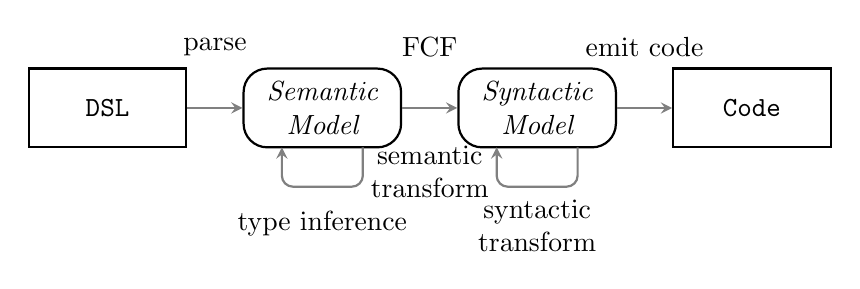
\begin{tikzpicture}[
  node distance=7mm,
  ,>=stealth,thick,black!50,text=black,
  every new ->/.style={shorten >=1pt}
]
  \node (dsl)  [resource]                                 {DSL};
  \node (sm)   [representation,right=of dsl,align=center] {Semantic\\Model};
  \node (cm)   [representation,right=of sm,align=center]  {Syntactic\\Model};
  \node (code) [resource,right=of cm]        {Code};


  \draw [->] (dsl) -> (sm)   node [midway,above=15pt]              {parse};
  \draw [->] (sm)  -> (cm)   node [midway,below=10pt,align=center] {semantic\\transform}
                             node [midway,above=15pt,align=center] {FCF};
  \draw [->] (cm)  -> (code) node [midway,above=15pt]              {emit code};

  \draw [rounded corners,->]
        ($ (sm.east) - (5mm,5mm) $)
        -- ++(0,-.5)
        -| ($ (sm.west) + (5mm,-5mm) $)
           node [near start, below=5pt] {type inference};

  \draw [rounded corners,->]
        ($ (cm.east) - (5mm,5mm) $)
        -- ++(0,-.5)
        -| ($ (cm.west) + (5mm,-5mm) $)
           node [near start, below=1pt,align=center] {syntactic\\transform};

\end{tikzpicture}
}
\caption{\FOO's code generation process}
\label{fig:code-generation}
\end{figure}

\vspace{-1mm}
\subsubsection{Semantic Model}

The semantic model is the core of the generator. It offers a way to describe
algorithms so that semantic reinterpretation through FCF is possible. This
reorganization of the functionality of different algorithms allows for more
optimal execution and memory usage. Hence the name \FOO of the framework:
functionality organization optimization. Figure \ref{fig:meta-model} shows the
central part of the semantic model as implemented for \FOO.\@ The concept driving
this model is the structure starting at the \emph{Model} up to the
\emph{Execution Strategy}. This structure encompasses the \emph{Function}s and
underlying \emph{Statement}s and allows for interpretation and fusion of the
algorithms.

\begin{figure}[b]
  \centering
  \scalebox{.75}{
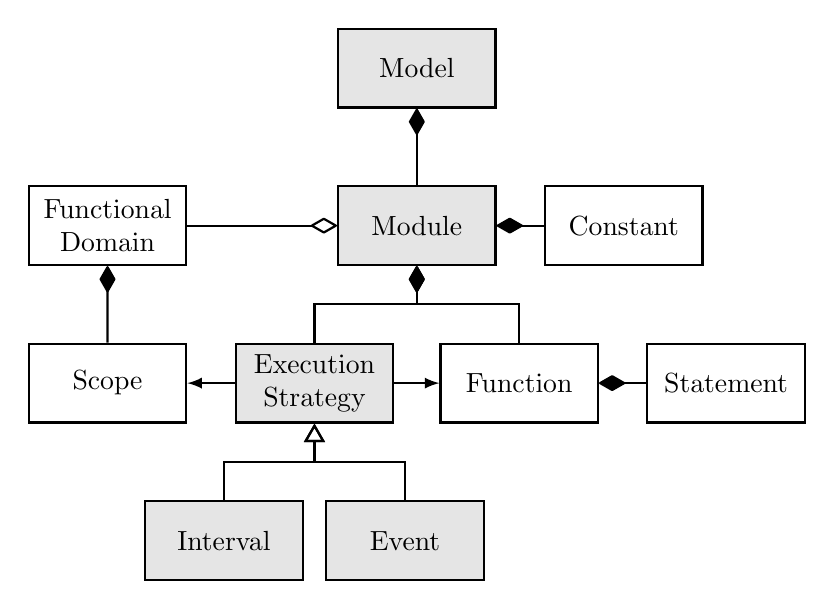
\begin{tikzpicture}[
  edge from parent fork down,
  sibling distance=5mm, level distance=20mm, node distance=6mm
  ]
  \node (model) [class,fill=black!10!white] {Model}
      child {node (module) [class,fill=black!10!white] {Module} edge from parent [composite]
        child {node (strategy) [class,align=center,xshift=-10.5mm,fill=black!10!white] {Execution\\Strategy} edge from parent [composite]
          child {node(every) [class,xshift=-9mm,fill=black!10!white] {Interval} edge from parent [subclass]}
          child {node (when) [class,xshift=9mm,fill=black!10!white] {Event} edge from parent [subclass]}
        }
        child {node (function) [class,xshift=10.5mm] {Function} edge from parent [composite]}
      };
  \node (constant)  [class,right=of module]                {Constant};
  \node (scope)     [class,left=of strategy]               {Scope};
  \node (statement) [class,right=of function]              {Statement};
  \node (domain)    [class,left=of module,xshift=-13mm]    {Functional\\Domain};
  
  \draw [aggregate]  (module)   -- (domain);
  \draw [composite]  (module)   -- (constant);
  \draw [dependency] (strategy) -- (scope);
  \draw [composite]  (function) -- (statement);
  
  \draw [composite]  (domain)   -- (scope);
  \draw [dependency] (strategy) -- (function);
\end{tikzpicture}
}
\caption{Partial Semantic Model for \FOO.\@ Shaded classes indicate the
\emph{event/scheduling} construction around functions to allow interpretation
of the intended functionality.}
\label{fig:meta-model}
\end{figure}

\vspace{-1mm}
\subsubsection{Functional Code Fusion (FCF)}

Thanks to the functional description of events and the effects triggered by
them, the code generator is able to identify the same actions across different
algorithms. This way it is possible to extract the parsing of incoming messages
and group actions on the same sets of data or scheduled function executions.
FCF typically looks for patterns in the semantic model and performs model
transformations to change these patterns to a more optimized organization. It
first performs semantic transformations on the semantic model itself. A second
phase transforms the semantic model into a syntactic model, encoding the
semantics into technical syntax constructs. One example of a semantic
transformation is type inference, which supports the platform independence of
the framework.

\vspace{-1mm}
\subsubsection{Syntactic Model}

The syntactic model is like an abstract syntax tree (AST) for a virtual,
expressive language. It contains constructs and ideas found in different
languages and programming paradigms. No single existing programming language
supports all features as is. Syntactic transformations therefore translate the
unsupported constructs into comparable constructs supported by the targeted
platform and language. Depending on the target platform, some constructions
aren't transformed into actually corresponding code. In selected cases, the
generator uses a software library. For example when it needs to parse incoming
messages or schedule tasks. During the generation process, it looks for
patterns that indicate any of these actions and transforms them into calls to
the \FOO software library.

\vspace{-1mm}
\subsection{\FOO as a Software Library}
\label{software-lib-design}

A software library allows offloading of common implementation aspects, thus
avoiding small discrepancies in code and suboptimal use of shared resources.
Previously we illustrated this approach with a case for unified messaging:
parsing of incoming messages and grouping of outgoing messages. More common
functionality isn't generated verbatim either. The execution of functions based
on a schedule or the implementation of higher level conceptual functions are
calls into the standard software library. Optimization of such algorithms is
not within the scope of \FOO.\@ This gives freedom of choice to the users of
the framework to select appropriate implementations for this standard
functionality.

\section{Implementation and Evaluation: Case Study on Intrusion Detection in Wireless Sensor Networks}
\label{evaluation}

In wired networks, firewalls focus on the outer perimeter of the network,
filtering unwanted packets. Still, attacks on services can pass unnoticed. This
is where an Intrusion Detection System (IDS) comes into play: monitoring all
traffic that passes through the firewall, looking for patterns of malicious
activity\cite{denning1987intrusion}. In meshed networks it is not possible for
a single point in the network to oversee all traffic
\cite{mishra2004intrusion}. Every device has to implement its own IDS.

Attackers have access to a large set of possible attack vectors
\cite{aschenbruck2012security}, ranging from the physical layer up to the
application layer. Each layer presents different opportunities for launching an
attack. For each of these attacks an algorithm needs to look for patterns or
anomalies. An IDS therefore requires a many algorithms to achieve adequate
coverage.

\vspace{-1mm}
\subsection{Implementation}

To evaluate the prototype we used a system based on the Atmel ATMEGA1284p
micro-controller and the Digi XBee S2 ZigBee module, running no specialized
operating system. Relying on basic hardware and software allows us to validate
that the generator is capable of generating code even for the most basic
environment. For the evaluation we constructed a small meshed network. In this
network, not all devices have direct access to one another, requiring routing
through shared neighboring devices.

We started from a basic application that measures light intensity. The
application was an includable piece of code, allowing integration in a both a
manual implementation and generated code base. On top of this baseline we added
two intrusion detection related algorithms: a watchdog
\cite{mishra2004intrusion}, that allows nodes to validate each other's
presence, and a reputation-based algorithm \cite{ganeriwal2008reputation}, that
checks if a parent node is cooperative and actually forwards messages.

\vspace{-1mm}
\subsection{Analytical Results}

Looking at the generated source code, a simple metric is comparing the amount
of code versus the size of the formal description of ID algorithms.
Implementing both algorithms manually results in 637 lines of C code. The
corresponding \FOO implementation requires only 156 lines of DSL code. Looking
at data structures, we see that sharing data eliminates redundant information,
such as a network address. This reduces the memory footprint for one node entry
by 2 bytes, from 27 bytes to 25 bytes. In our implementation we used the ZigBee
network address, which consists of 16 bits. This results in a reduction of
7.4\% of dynamic memory per known device. Using ZigBee's 64 bits unique
addresses, this reduction can easily become 20.5\%.

\vspace{-1mm}
\subsection{Experimental Results}

We also instrumented the code and evaluated four criteria: network usage
(number of packets and bytes), the time required to perform once cycle of the
event loop and the resulting image size. We collected these metrics for four
situations: without ID algorithms, with a watchdog, with reputation-tracking
and with both algorithms. The manual implementation realized both algorithms as
standalone modules and sequentially called them from the base-application's
event loop. Given the \FOO descriptions of the algorithms, the code generator
generated all four cases. Table \ref{tbl:results} shows the collected data.

\begin{table}[h]
  \caption{Experimental Results and Side-by-Side Comparison.}
  \label{tbl:results}
\begin{tabular*}{\hsize}{@{\extracolsep{\fill}}llrrrrrrr@{}}
\toprule
              &            & base  & \multicolumn{2}{c}{watchdog} & \multicolumn{2}{c}{reputation} & \multicolumn{2}{c}{both} \\
\midrule
\multirow{2}{*}{\pbox{\textwidth}{total packets sent\\in a window of 90s}}
              & manual     &    20 &    51 & +155\% &    32 &  +60\% &    63 & +215\%\\
              & generated  &    20 &    49 & +145\% &    32 &  +60\% &    55 & +175\%\\
\cmidrule{2-9}
              & difference &     0 &    -2 &   -4\% &     0 &   0\% &    -8 &   -13\%\\
\midrule
\multirow{2}{*}{\pbox{\textwidth}{total bytes sent\\in a window of 90s}}
              & manual     &   476 &  1933 & +306\% &   860 &  +81\% &  2317 & +387\%\\
              & generated  &   476 &  1897 & +299\% &   884 &  +86\% &  2161 & +354\%\\
\cmidrule{2-9}
              & difference &     0 &   -36 &   -2\% &    24 &   +3\% &  -156 &   -7\%\\
\midrule
\multirow{2}{*}{\pbox{\textwidth}{event loop\\average duration ($\mu$s)}}
              & manual     &    48 &    94 &  +96\% &    88 &  +83\% &   149 & +210\%\\
              & generated  &    48 &   121 & +152\% &   121 & +152\% &   138 & +188\%\\
\cmidrule{2-9}
              & difference &     0 &    27 &  +29\% &    33 &  +38\% &   -11 &   -7\%\\
\midrule
image
size (bytes)  & manual     & 10466 & 15530 &  +48\% & 13306 &  +27\% & 18334 &  +75\%\\
              & generated  & 10466 & 18352 &  +75\% & 16376 &  +56\% & 20998 & +101\%\\
\cmidrule{2-9}
              & difference &     0 &  2822 &  +18\% &  3070 &  +23\% &  2664 &  +15\%\\
\bottomrule
  \end{tabular*}
\end{table}

These results show that adding algorithms manually to the base-application has
a cumulative effect. In case of the generated implementation, this effect is no
longer observed: individual algorithms do have a larger impact by themselves,
but the combination of both algorithms is less than the sum of both. Most
remarkable is the effect on the time of one event loop cycle: both algorithms
by itself add 152\%. Adding a second algorithm only augments the impact to
188\%. We see the effect of the generic handling of common functionality. It
comes with an overhead for a single algorithm, but pays for itself when adding
more algorithms.

Table \ref{tbl:results} also compares the two situations, showing the impact of
the code generation: Both the number of packets as well as the amount of bytes
sent have dropped by 13\% and 7\%. In case of the execution time, both
algorithms by themselves add an equal amount of time to a single event loop
cycle. When combined, the event loop is about 7\% faster compared to the manual
case. Finally, we see that the software library adds to the size of the
resulting image. However, the cost is close to constant and is lower for both
algorithms together. With roughly 3KB of additional overhead, or 15\% in this
simple case, the impact is small. Taking into account the available memory on
the ATMega1284p, this is only 2.3\% of the available resources.

\section{Related Work}
\label{related}

This section focuses on related work in the field of domain specific languages
and code generation, in relation to wireless networks of resource-constrained
devices. These two components are the core of the \FOO framework.

Within the scope of wireless networks of resource-constrained devices, we see
the introduction of DSLs \enquote{to shorten the development cycles
dramatically during deployments, to reduce the dependency on hardware and
software engineers, and to lead to a wider adoption outside the computer
science field} \cite{sadilek2008domain}. TinyScript \cite{levis2004tinyscript}
is an example of a language for wireless sensor networks. It's a complete
programing language that aims to ease the description of algorithms in general.
The Basic-like syntax does enable more productive development. Still, this
approach doesn't address the underlying resource problems inherently connected
to the context. SEAL \cite{elsts2013seal} is a novel complete programming
language that focuses on novice programmers. It is a clear fit for
\emph{sense-and-send} type of applications. It does however share the idea of
using events to overcome the technical nature of loops. In the context of
intrusion detection, we learn that DSLs are predominantly used to describe
patterns of events found in network packets
\cite{sekar1999high,roesch1999snort} in a concise way. The STAT framework with
its STATL language \cite{eckmann2002statl,vigna2003designing} allow to model
scenarios using state machines. Our event-driven approach shares these same
ideas. Although not a real DSL, nesC \cite{gay2003nesc} is a general purpose
language that shares some typical concepts with \FOO, such as the high degree
of analysis during code generation to optimize execution. The biggest
difference is that \FOO starts from the intended functionality and can optimize
certain constructions that can't be interpreted from more technical source code.

Code generation, in combination with a DSL, can optimize a development process
by reducing the size of the code base or systematically improving the code
quality. Embedded systems are a prime example of an environment where code
needs to be of a high quality. Focus on size and performance are a logical
choice when dealing with limited storage and processing power. Compilers
implement different techniques to address this at the lowest level
\cite{marwedel2002code}. Optimizing for power efficiency however proves to be
concurrent to size and performance optimization, and requires different
strategies. Data and memory optimizations \cite{panda2001data} can result in
improvements on a lower level. To really preserve energy one requires
higher-level strategies, targeting architecture, radio handling, efficient
software,\dots \cite{naik2001software}. Most of these are beyond the control of
the compiler and require a higher level of abstraction to address them. DSLs
offer a solution here, but other paradigms are possible. A mixed framework
consisting of a virtual machine (VM) and native code extension
\cite{sadilek2007energy}, combined with energy-aware compilation, seems a
promising approach. By offloading the optimization to a VM and only compiling
parts and not the whole, the solution allows updating at a granular scale, thus
reducing the update cost, while maintaining flexibility and lowering the
development effort. In this terminology, \FOO focuses on the reduction of the
development effort and update cost, and maximizes flexibility.

\section{Conclusion and Future Work}
\label{conclusion}

Many IoT applications typically are constructed of similar algorithms that
adhere to a pattern of collecting sensor data and periodically checking
recorded values for patterns that require action. Fusing these algorithms is
hard but needed to deal with the resource-constrained devices they are
targeting. Frequent reselection, e.g. due to changing requirements or changing
security threats, requires a flexible way to incorporate these algorithms in
subsequent iterations of the software.

\FOO is a framework consisting of a DSL, a source code generator and software
library. The DSL allows formally describing algorithms, enabling the code
generator to apply functional code fusion to interpret the intent of algorithms
and merge common functionality \& shared data. The software library hosts
common functionality, such as sensor access, message parsing and event
scheduling. The platform independent DSL enables generation of source code
targeting different platforms and languages, which allows high degrees of reuse
with heterogenous devices.

Initial experiments confirm the theoretically positive impact on resource
usage: grouping of messages lowers the number of packets by 13\%, while the
total number of bytes sent over the network is reduced by 7\%. The execution
time is improved by 7\% and memory usage can be reduced by even 20\%.

Future research will focus on the integration of applications with the
generated functionality. We see opportunities for applications to adopt the
event-driven approach and hope to expand the capabilities of \FOO to this
level. A continued effort is targeting the reduction of platform-dependent
parts in the implementation. This way it is possible to add more platforms and
languages with less effort. In the longer run, we want to investigate the
possibility to extend the functional code fusion paradigm to more domains.

\section{Acknowledgements}

This research is partially funded by the Research Fund KU Leuven and partially
by the EU FP7 project NESSoS\@.

\bibliographystyle{elsarticle-num}
\bibliography{literature/referenties}

\end{document}
